\subsection{Backend}

The following section will describe how the NetInf NRS application will be evaluated and tested. One of the goals of the project was to show that the use of the new Network of Information protocol (NetInf) would be better in terms of bandwidth, speed and time compared to existing location based infrastructure. 

The Erlang NetInf NRS application, along with the video stream was evaluated with the following set of tests. 


\subsubsection{Video streaming protocol evaluation}
The client requested the development team to look into the application of NetInf to real world problems, one of the problems discussed was reducing congestion for broadcasting content. This was solved by implementing an alternative way of sending chunked data as seen in Section \ref{sec:Chunked data streaming} according to the video streaming draft seen in Appendix \ref{VideoDraft}. In the following section this implementation is called the modified streaming. The following was test was conducted:

\begin{itemize}
\item Testing the modified version of NetInf video streaming. 
\item Testing the pure version of NetInf video streaming.
\item Comparison between both implementations of the NetInf Video streaming
\end{itemize}

The testing was done by transferring 500 chunks of bogus data between a number of different NetInf nodes running ERNI. All the receiving nodes started the transfer at the same time. To be able to publish N number of chunks in an easy and fast manner, the \textit{nn\_evaluation} module was implemented.

%The backbone of the entire application, this is the main product which the client requested. It is important to show here just how much better this implementation of NetInf is compared to location based services used today. 

\subsubsection{Pure video streaming evaluation setup}
The nodes that were included in the pure version of the streaming was the following. 
Central NRS which all NDOs the without octects where published. 
One source node that publish all 500 NDOs to itself with \textit{fullput} set to true, then also publish the NDO to the central NRS with \textit{fullput} false. The central NRS can not have the octets because otherwise it would provide all clients with the octects directly, hence prevent the network load to be more balanced.
Five clients nodes then got each chunk by:
\begin{enumerate}
\item search NRS for the chunk with chunk number and stream name.
\item get the NDO metadata and locators from the NRS.
\item fetch NDO with octects from one of the locators.
\item add itself as a locator and publish to the NRS.
\item repeat the procedure for the next chunk.
\end{enumerate}

\subsubsection{Modified video streaming evaluation setup}
In this setup the nodes present was one that served as both the source and central NRS and five client nodes. The source first published the stream NDO to itself, then use the content dispatcher to put all the chunks in the storage.
The clients then get the stream NDO, add them self as locator and publish it. To retrieve the chunks each client need to:
\begin{enumerate}
\item append the current chunk number to the NDO name.
\item send the request to one of the locators.
\item if status of the response is 404, repeat step 2.
\item store the octects in its storage.
\item increase the chunk number
\end{enumerate}

\subsubsection{Stream results and comparison} 
The Figure~\ref{fig:eval-stream-modvspure} shows that the pure NetInf streaming is more efficient when it comes to transferring all the chunks. This result is not that unexpected since the modified version have a lot of over head in this case, if it tries to get a chunk from an other client which does not have them yet, this will yield in an 404 response and the client will need to try another source. While the pure NetInf will get a hit every time. 
 
When comparing Figure~\ref{fig:eval-stream-pure-cpu} and Figure~\ref{fig:eval-stream-mod-cpu}, it shows that even with only five receiving nodes the central NRS is struggling with the searches. While the CPU load of the modified version is almost not noticeable.  

\begin{figure}[h!]
	\centering
		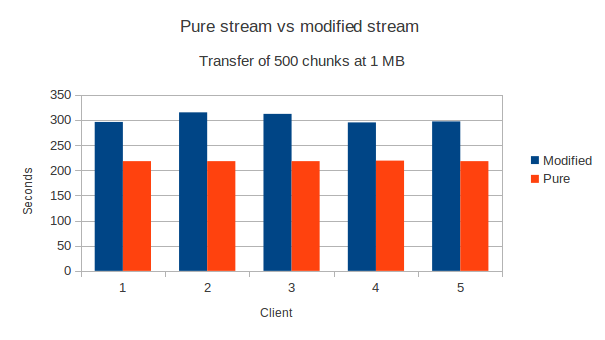
\includegraphics[width=0.75\textwidth]{./img/eval-stream-plot-modvspure.png}
    	\caption{Pure streaming vs modified streaming}
	\label{fig:eval-stream-modvspure}
\end{figure}

\begin{figure}[h!]
	\centering
		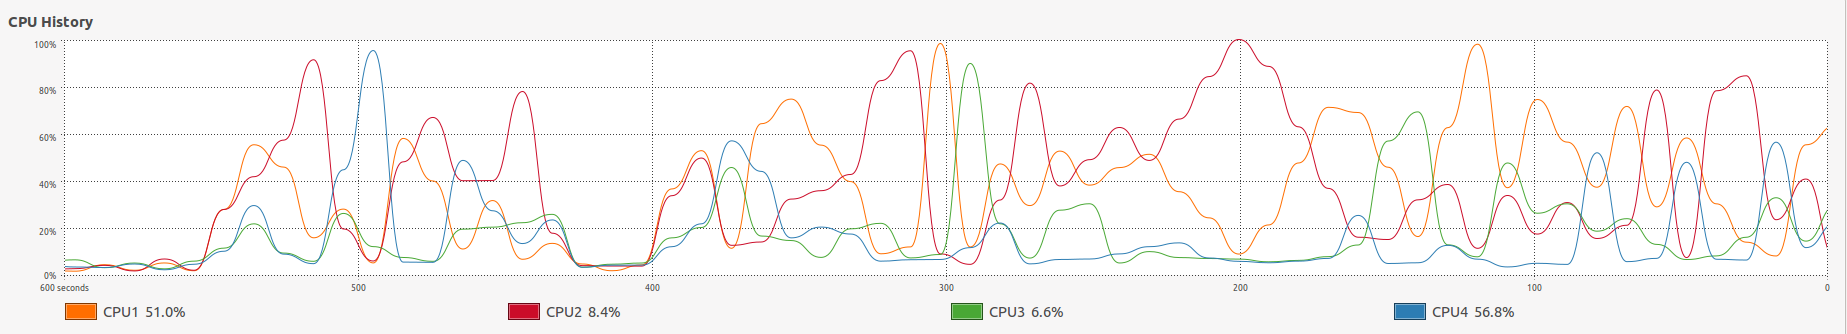
\includegraphics[width=0.75\textwidth]{./img/eval-stream-pure-cpu.png}
    	\caption{Central NRS CPU usage during pure streaming}
	\label{fig:eval-stream-pure-cpu}
\end{figure}

\begin{figure}[h!]
	\centering
		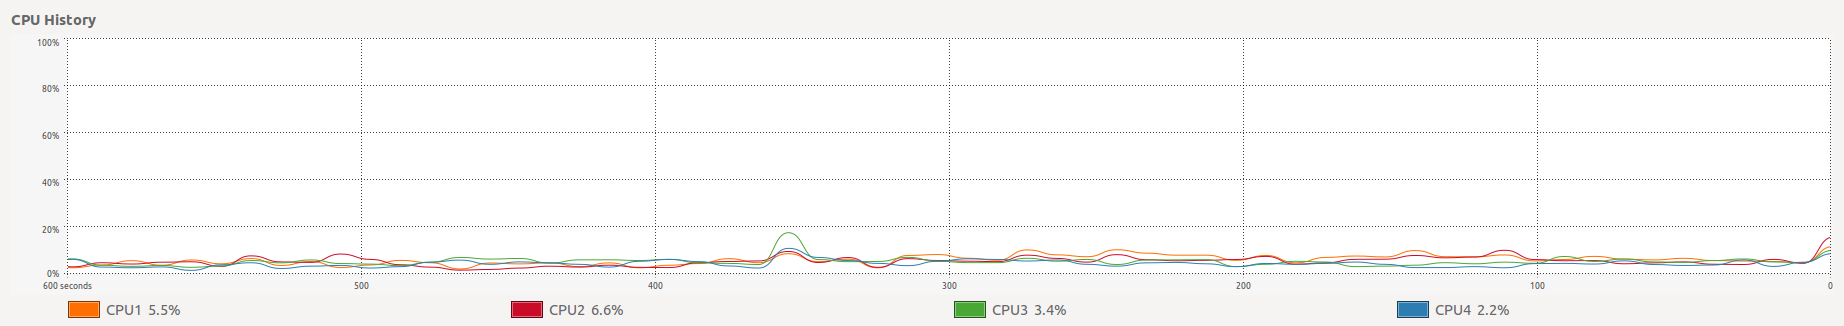
\includegraphics[width=0.75\textwidth]{./img/eval-stream-mod-cpu.png}
    	\caption{Central NRS CPU usage during modified streaming}
	\label{fig:eval-stream-mod-cpu}
\end{figure}



\subsubsection{Notes on Interoperability}

There already are existing implementations done by SAIL and Ericsson Research for the NetInf protocol and in the beginning of the product life-cycle the client requested the development team to try to evaluate the interoperability of this product and others, however as the product evolved the client's requested that the interoperability be left to them to evaluate and for this development team to continue with evaluating the video streaming.

Therefore the development team did not evaluate interoperability at all but there is confidence that with some minor tweaking of the code (due to differences in the various draft versions of the NetInf protocol spec) that this product and others will become interoperable with minimal effort.


\begin{itemize}
\item Evaluation of the search time and get time for the supported databases
\item Resource usage
\item Measuring the number of requests per the frontend phone client
\end{itemize}
